Data from the given question is available in Table \ref{constr/circ/61/tab:table1}:
%
\begin{table}[!ht]
\begin{center}
\begin{tabular}{ | m{2cm} | m{1.5cm}| m{2cm} | m{1.5cm} |} 
\hline
& Symbols & Circle1  \\
\hline
Centre & $\vec{C}$ & \myvec{0\\0}  \\ 
\hline
Radius & $r$& 3.4 \\ 
\hline
\end{tabular}
\end{center}
\caption{Input values}
\label{constr/circ/61/tab:table1}
\end{table}
%
Let 
\begin{align}
      \vec{P} &= r \myvec{\cos \theta_1\\ \sin \theta_1} =  \myvec{1.7\\2.9}
      \\
      \vec{Q} &= r \myvec{\cos \theta_2\\ \sin \theta_2} =\myvec{-2.4\\2.4}
 \end{align}
 Then the perpendicular bisector of $PQ$ passes through 
 \begin{align}
    \vec{M} = \frac{\vec{P}+\vec{Q}}{2} 
\end{align}
and has normal vector 
\begin{align}
    \vec{n} = \vec{P}-\vec{Q}
\end{align}
resulting in the equation
\begin{align}
    \brak{\vec{P}-\vec{Q}}^\top\brak{\vec{x}-\frac{\vec{P}+\vec{Q}}{2} } = 0
    \implies \brak{\vec{P}-\vec{Q}}^\top\vec{x} = 0
\end{align}
%
after simplification.  It is obvious that $\vec{O}$ satisfies the above equuation as can be verified in Fig.     \ref{constr/circ/61/fig: perpenicular bisector of the chord passes through the center}.
%
\begin{figure}[ht]
    \centering
    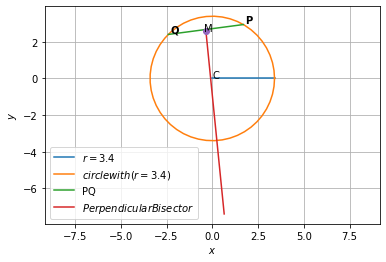
\includegraphics[width=\columnwidth]{solutions/circle/61/FIG.3.png}
    \caption{perpendicular bisector of the chord passes through the center}
    \label{constr/circ/61/fig: perpenicular bisector of the chord passes through the center}
\end{figure}






